\documentclass[xetex,mathserif,serif]{beamer}
\usepackage{polyglossia}
\setdefaultlanguage[babelshorthands=true]{russian}
\usepackage{listings}
\usepackage{tabu}

\useoutertheme{infolines}

\usepackage{fontspec}
\setmainfont{FreeSans}
\newfontfamily{\russianfonttt}{FreeSans}

\setbeamertemplate{blocks}[rounded][shadow=false]
\setbeamercolor*{block title example}{fg=green!50!black,bg=green!20}
\setbeamercolor*{block body example}{fg=black,bg=green!10}

\setbeamercolor*{block title alerted}{fg=red!50!black,bg=red!20}
\setbeamercolor*{block body alerted}{fg=black,bg=red!10}

\lstset{language=Caml,basicstyle=\small\normalfont,keywordstyle=\color{red},showstringspaces=false}

\lstset{emph={member,float,int,static,open,class,val,new,inherit,abstract,override,default,base,interface,int,bool,unit,string,module,struct,namespace,return,public,throw,use,finally,elif},emphstyle={\color{red}},deletekeywords={value}}

\DeclareMathSymbol{\mlq}{\mathord}{operators}{``}
\DeclareMathSymbol{\mrq}{\mathord}{operators}{`'}

\tabulinesep=1.2mm

\title{Низкоуровневые потоки, события}
\author{Юрий Литвинов}
\date{06.05.2016г}

\begin{document}

    \frame{\titlepage}

    \begin{frame}
        \frametitle{Управление потоками ``вручную''}
        \begin{itemize}
            \item Сложнее и опаснее, чем async
            \item Позволяет управлять приоритетом потока, делать поток 
                foreground или background, точнее управлять временем жизни
                и поведением потока, использовать низкоуровневые механизмы
                синхронизации
            \item Абстракция отдельного ядра, а не асинхронного вычисления
        \end{itemize}
    \end{frame}
    
    \begin{frame}[fragile]
        \frametitle{Класс System.Threading.Thread}
        \begin{exampleblock}{F\#}
            \begin{lstlisting}
open System.Threading

let t = new Thread(ThreadStart(fun _ ->
    printfn "Thread %d: Hello" 
            Thread.CurrentThread.ManagedThreadId))

t.Start()
printfn "Thread %d: Waiting!" 
            Thread.CurrentThread.ManagedThreadId
t.Join()
printfn "Done!"
\end{lstlisting}
\end{exampleblock}
\end{frame}

    \begin{frame}
        \frametitle{Потенциальные проблемы с потоками}
        \begin{itemize}
            \item Гонки (Race condition)
                \begin{center}
                    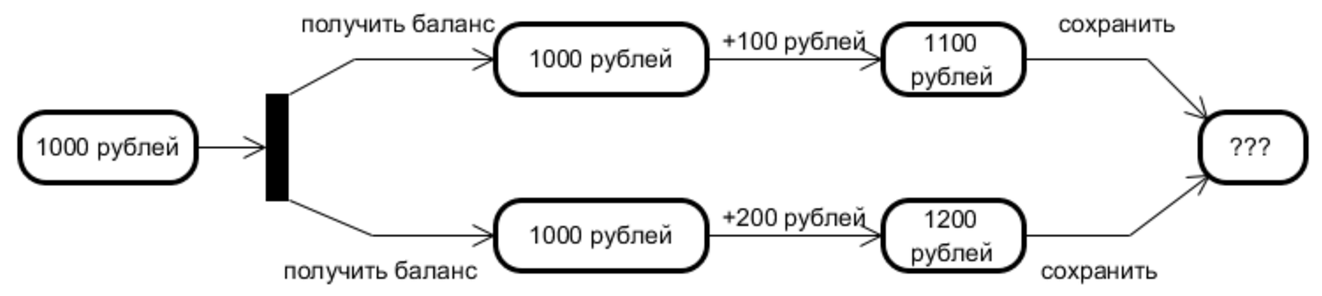
\includegraphics[width=0.8\textwidth]{raceCondition.png}
                \end{center}
                \vspace{1cm}
            \item Тупики (Deadlock)
                \begin{center}
                    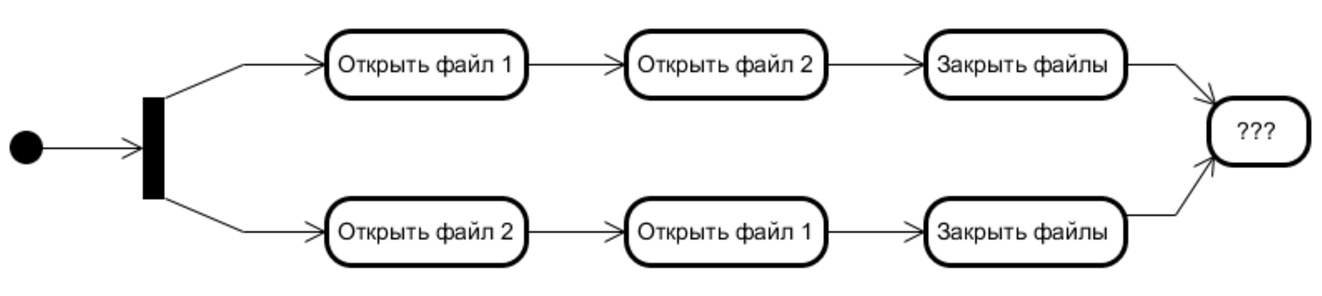
\includegraphics[width=0.8\textwidth]{deadlock.png}
                \end{center}
        \end{itemize}
    \end{frame}
    
    \begin{frame}[fragile]
        \frametitle{Пример гонки}
        \begin{exampleblock}{F\#}
            \begin{lstlisting}
type MutablePair<'a,'b>(x:'a, y:'b) =
    let mutable currentX = x
    let mutable currentY = y
    member p.Value = (currentX, currentY)
    member p.Update(x, y) =
        currentX <- x
        currentY <- y

let p = MutablePair (0, 0)
Async.Start (async { while true do p.Update(10, 10) })
Async.Start (async { while true do p.Update(20, 20) })

Async.RunSynchronously (async { while true do () })
\end{lstlisting}
\end{exampleblock}
\end{frame}

    \begin{frame}[fragile]
        \frametitle{Пример примитива синхронизации: монитор}
        \begin{exampleblock}{F\#}
            \begin{lstlisting}
let lock (lockobj : obj) f =
    Monitor.Enter lockobj
    try
        f()
    finally
        Monitor.Exit lockobj

Async.Start (async { 
    while true do lock p (fun () -> p.Update(10, 10)) })

Async.Start (async { 
    while true do lock p (fun () -> p.Update(20, 20)) })
\end{lstlisting}
\end{exampleblock}
\end{frame}

    \begin{frame}
        \frametitle{Примитивы синхронизации}
        \framesubtitle{Пространство имён System.Threading}
        \begin{footnotesize}
            \begin{tabu} {| X[0.3 l p] | X[1 l p] |}
                \tabucline-
                Примитив                 & Описание           \\
                \tabucline-
                \everyrow{\tabucline-}
                AutoResetEvent    & Точка синхронизации. WaitOne блокирует поток, пока кто-нибудь другой не вызовет Set.  \\
                ManualResetEvent  & То же, что AutoResetEvent, но сбрасывается вручную, вызовом Reset                     \\
                Monitor           & Ограничивает доступ к критической секции                                              \\
                Mutex             & Ограничивает доступ к критической секции, работает между процессами                   \\
                Semaphore         & Позволяет находиться в критической секции не более N потоков                          \\
                Interlocked       & Атомарные арифметические операции                                                     \\
            \end{tabu}
        \end{footnotesize}
    \end{frame}

    \begin{frame}[fragile]
        \frametitle{BackgroundWorker}
        \framesubtitle{Более высокоуровневый способ работы с потоками}
        \begin{exampleblock}{F\#}
            \begin{lstlisting}
let worker = new BackgroundWorker()
let numIterations = 1000

worker.DoWork.Add(fun args ->
    let rec computeFibonacci resPrevPrev resPrev i =
        let res = resPrevPrev + resPrev
        
        if i = numIterations then
            args.Result <- box res
        else
            computeFibonacci resPrev res (i + 1)

    computeFibonacci 1 1 2)
\end{lstlisting}
\end{exampleblock}
\end{frame}

    \begin{frame}[fragile]
        \frametitle{BackgroundWorker, как запустить}
        \begin{exampleblock}{F\#}
            \begin{lstlisting}
worker.RunWorkerCompleted.Add(fun args ->
    MessageBox.Show (sprintf "Result = %A" 
        args.Result) |> ignore)

worker.RunWorkerAsync()
\end{lstlisting}
\end{exampleblock}
\end{frame}

    \begin{frame}[fragile]
        \frametitle{События}
        \begin{alertblock}{F\# Interactive}
            \begin{lstlisting}[keywordstyle=\color{black},emphstyle=\color{black}]
> open System.Windows.Forms;;
> let form = new Form(Text="Click Form",  
                      Visible=true,TopMost=true);;
val form : Form

> form.Click.Add(fun evArgs -> printfn "Clicked!");;
val it : unit = ()

> form.MouseMove.Add(fun args -> printfn "Mouse, 
                     (X,Y) = (%A,%A)" args.X args.Y);;
val it : unit = ()
\end{lstlisting}
\end{alertblock}
\end{frame}

    \begin{frame}[fragile]
        \frametitle{Microsoft.FSharp.Control.Event}
        \begin{exampleblock}{F\#}
            \begin{lstlisting}
Form.MouseMove
    |> Event.filter (fun args -> args.X > 100)
    |> Event.add (fun args -> printfn "Mouse, 
                  (X,Y) = (%A,%A)" args.X args.Y)
\end{lstlisting}
\end{exampleblock}
\end{frame}

    \begin{frame}
        \frametitle{Что ещё с ними можно делать}
        \begin{footnotesize}
            \begin{tabu} {| X[0.3 l p] | X[1 l p] |}
                \tabucline-
                Примитив  & Описание           \\
                \tabucline-
                \everyrow{\tabucline-}
                add       & ('T $\to$ unit) $\to$ IEvent<'Del,'T> $\to$ unit                                 \\
                filter    & ('T $\to$ bool) $\to$ IEvent<'Del,'T> $\to$ IEvent<'T>                           \\
                choose    & ('T $\to$ 'U option) $\to$ IEvent<'Del,'T> $\to$ IEvent<'U>                      \\
                map       & ('T $\to$ 'U) $\to$ IEvent<'Del, 'T> $\to$ IEvent<'U>                            \\
                merge     & IEvent<'Del1,'T> $\to$ IEvent<'Del2,'T> $\to$ IEvent<'T>                         \\
                pairwise  & IEvent<'Del,'T> $\to$ IEvent<'T * 'T>                                            \\
                partition & ('T $\to$ bool) $\to$ IEvent<'Del,'T> $\to$ IEvent<'T> * IEvent<'T>              \\
                scan      & ('U $\to$ 'T $\to$ 'U) $\to$ 'U $\to$ IEvent<'Del,'T> $\to$ IEvent<'U>           \\
                split     & ('T $\to$ Choice<'U1,'U2>) $\to$ IEvent<'Del,'T> $\to$ IEvent<'U1> * IEvent<'U2> \\
            \end{tabu}
        \end{footnotesize}
    \end{frame}
    
    \begin{frame}[fragile]
        \frametitle{Как описывать свои события}
        \begin{exampleblock}{F\#}
            \begin{lstlisting}
open System
open System.Windows.Forms

type RandomTicker(approxInterval) =
    let timer = new Timer()
    let rnd = new System.Random 99
    let tickEvent = new Event<_>()

    let chooseInterval() :int =
        approxInterval + approxInterval / 4
               - rnd.Next(approxInterval / 2)

    do timer.Interval <- chooseInterval()
\end{lstlisting}
\end{exampleblock}
\end{frame}

    \begin{frame}[fragile]
        \frametitle{Как описывать свои события (2)}
        \begin{exampleblock}{F\#}
            \begin{lstlisting}
do timer.Tick.Add(fun args ->
    let interval = chooseInterval()
    tickEvent.Trigger(interval)
    timer.Interval <- interval)

member x.RandomTick = tickEvent.Publish
member x.Start() = timer.Start()
member x.Stop() = timer.Stop()

interface IDisposable with
    member x.Dispose() = timer.Dispose()
\end{lstlisting}
\end{exampleblock}
\end{frame}

    \begin{frame}[fragile]
        \frametitle{Пример использования}
        \begin{alertblock}{F\# Interactive}
            \begin{lstlisting}[keywordstyle=\color{black},emphstyle=\color{black}]
> let rt = new RandomTicker(1000);;
val rt : RandomTicker
> rt.RandomTick.Add(fun nextInterval -> printfn "Tick, 
        next = %A" nextInterval);;
val it : unit = ()

> rt.Start();;
Tick, next = 1072
Tick, next = 927
Tick, next = 765
...
val it : unit = ()
> rt.Stop();;
val it : unit = ()
\end{lstlisting}
\end{alertblock}
\end{frame}

    \begin{frame}[fragile]
        \frametitle{Свой worker, с событиями}
        \begin{exampleblock}{F\#}
            \begin{lstlisting}
open System.ComponentModel
open System.Windows.Forms

type IterativeBackgroundWorker<'a>(oneStep:('a -> 'a),
        initialState:'a,
        numIterations:int) =
    let worker =
        new BackgroundWorker(WorkerReportsProgress=true,
            WorkerSupportsCancellation=true)

    let completed = new Event<_>()
    let error = new Event<_>()
    let cancelled = new Event<_>()
    let progress = new Event<_>()
\end{lstlisting}
\end{exampleblock}
\end{frame}

    \begin{frame}[fragile]
        \frametitle{Свой worker (2)}
        \begin{exampleblock}{F\#}
            \begin{lstlisting}
do worker.DoWork.Add(fun args ->
let rec iterate state i =
    if worker.CancellationPending then
        args.Cancel <- true
    elif i < numIterations then
        let state' = oneStep state
        let percent = int ((float (i + 1) 
            / float numIterations) * 100.0)
        do worker.ReportProgress(percent, box state);
        iterate state' (i+1)
    else
        args.Result <- box state

iterate initialState 0)
\end{lstlisting}
\end{exampleblock}
\end{frame}

    \begin{frame}[fragile]
        \frametitle{Свой worker (3)}
        \begin{exampleblock}{F\#}
            \begin{lstlisting}[basicstyle=\scriptsize]
do worker.RunWorkerCompleted.Add(fun args ->
    if args.Cancelled then cancelled.Trigger ()
    elif args.Error <> null then error.Trigger args.Error
    else completed.Trigger (args.Result :?> 'a))

do worker.ProgressChanged.Add(fun args ->
    progress.Trigger (args.ProgressPercentage, (args.UserState :?> 'a)))

member x.WorkerCompleted = completed.Publish
member x.WorkerCancelled = cancelled.Publish
member x.WorkerError = error.Publish
member x.ProgressChanged = progress.Publish

member x.RunWorkerAsync() = worker.RunWorkerAsync()
member x.CancelAsync() = worker.CancelAsync()
\end{lstlisting}
\end{exampleblock}
\end{frame}

    \begin{frame}[fragile]
        \frametitle{Тип того, что получилось}
        \begin{exampleblock}{F\#}
            \begin{lstlisting}
type IterativeBackgroundWorker<'a> =
  class
    new : oneStep:('a -> 'a) 
            * initialState:'a 
            * numIterations:int 
            -> IterativeBackgroundWorker<'a>
    member CancelAsync : unit -> unit
    member RunWorkerAsync : unit -> unit
    member ProgressChanged : Event<int * 'a>
    member WorkerCancelled : Event<unit>
    member WorkerCompleted : Event<'a>
    member WorkerError : Event<exn>
  end
\end{lstlisting}
\end{exampleblock}
\end{frame}

    \begin{frame}[fragile]
        \frametitle{Пример использования}
        \begin{exampleblock}{F\#}
            \begin{lstlisting}
let fibOneStep (fibPrevPrev:bigint,fibPrev) = 
                  (fibPrev, fibPrevPrev + fibPrev)

let worker = new IterativeBackgroundWorker<_>(fibOneStep,
             (1I, 1I), 100)

worker.WorkerCompleted.Add(fun result ->
  MessageBox.Show(sprintf "Result = %A" result) |> ignore)

worker.ProgressChanged.Add(fun (percentage, state) ->
  printfn "%d%% complete, state = %A" percentage state)

worker.RunWorkerAsync()
\end{lstlisting}
\end{exampleblock}
\end{frame}

    \begin{frame}[fragile]
        \frametitle{Своё новое событие}
        \begin{exampleblock}{F\#}
            \begin{lstlisting}[basicstyle=\scriptsize]
open System
open System.Threading

type IterativeBackgroundWorker<'a>(...) =
    let worker = ...

    let syncContext = SynchronizationContext.Current
    do if syncContext = null then failwith 
        "no synchronization context found"
    
    let started = new Event<_>()

    do worker.DoWork.Add(fun args ->
        syncContext.Post(SendOrPostCallback(fun _ -> 
            started.Trigger(DateTime.Now)),
            state=null))
    ...
    member x.Started = started.Publish
\end{lstlisting}
\end{exampleblock}
\end{frame}

    \begin{frame}[fragile]
        \frametitle{Большой пример (1)}
        \begin{exampleblock}{F\#}
            \begin{lstlisting}[basicstyle=\scriptsize]
open System.Drawing
open System.Windows.Forms

let form = new Form(Visible = false, TopMost = true)

let panel = new FlowLayoutPanel(Visible = true,
    Height = 20,
    Dock = DockStyle.Bottom,
    BorderStyle = BorderStyle.FixedSingle)

let progress = new ProgressBar(Visible = false,
    Anchor=(AnchorStyles.Bottom ||| AnchorStyles.Top),
    Value = 0)

let text = new Label(Text = "Paused",
    Anchor = AnchorStyles.Left,
    Height = 20,
    TextAlign = ContentAlignment.MiddleLeft)
\end{lstlisting}
\end{exampleblock}
\end{frame}

    \begin{frame}[fragile]
        \frametitle{Большой пример (2)}
        \begin{exampleblock}{F\#}
            \begin{lstlisting}[basicstyle=\scriptsize]
panel.Controls.Add(progress)
panel.Controls.Add(text)
form.Controls.Add(panel)

let fibOneStep (fibPrevPrev:bigint,fibPrev) = (fibPrev, fibPrevPrev+fibPrev)

// Run the iterative algorithm 500 times before reporting intermediate results
// Burn some additional cycles to make sure it runs slowly enough
let rec RepeatN n f s = if n <= 0 then s else RepeatN (n - 1) f (f s)
let rec BurnN n f s = if n <= 0 then f s else ignore (f s); BurnN (n - 1) f s
let step = (RepeatN 500 (BurnN 1000 fibOneStep))

// Create the iterative worker.
let worker = new IterativeBackgroundWorker<_>(step,(1I,1I),100)
\end{lstlisting}
\end{exampleblock}
\end{frame}

    \begin{frame}[fragile]
        \frametitle{Большой пример (3)}
        \begin{exampleblock}{F\#}
            \begin{lstlisting}[basicstyle=\scriptsize]
worker.ProgressChanged.Add(fun (progressPercentage,state)->
        progress.Value <- progressPercentage)

worker.WorkerCompleted.Add(fun (_,result) ->
        progress.Visible <- false;
        text.Text <- "Paused";
        MessageBox.Show(sprintf "Result = %A" result) |> ignore)

worker.WorkerCancelled.Add(fun () ->
        progress.Visible <- false;
        text.Text <- "Paused";
        MessageBox.Show(sprintf "Cancelled OK!") |> ignore)

worker.WorkerError.Add(fun exn ->
        text.Text <- "Paused";
        MessageBox.Show(sprintf "Error: %A" exn) |> ignore)
\end{lstlisting}
\end{exampleblock}
\end{frame}

    \begin{frame}[fragile]
        \frametitle{Большой пример (4)}
        \begin{exampleblock}{F\#}
            \begin{lstlisting}[basicstyle=\scriptsize]
form.Menu <- new MainMenu()
let workerMenu = form.Menu.MenuItems.Add("&Worker")

workerMenu.MenuItems.Add(new MenuItem("Run",onClick=(fun _ args ->
        text.Text <- "Running";
        progress.Visible <- true;
        worker.RunWorkerAsync()))) |> ignore

workerMenu.MenuItems.Add(new MenuItem("Cancel",onClick=(fun _ args ->
        text.Text <- "Cancelling";
        worker.CancelAsync()))) |> ignore

form.Closed.Add(fun _ -> worker.CancelAsync())

form.ShowDialog () |> ignore
\end{lstlisting}
\end{exampleblock}
\end{frame}

\end{document}
